\lab{Gradient Descent Methods}{Gradient Descent Methods}
\todoChapter{ Todo: Adapt and incorporate this material. }
\objective{Iterative optimization methods choose a search direction and a step size at each iteration.
One simple choice for the search direction is the negative gradient, resulting in the method of steepest descent.
While theoretically foundational, in practice this method is often slow to converge.
An alternative method, the conjugate gradient algorithm, uses a similar idea that results in much faster convergence in some situations.
In this lab we implement a method of steepest descent and two conjugate gradient methods, then apply them to regression problems.
}

\section*{The Method of Steepest Descent} % ===================================

Let $f:\mathbb{R}^n \rightarrow \mathbb{R}$ with first derivative $Df:\mathbb{R}^n \rightarrow \mathbb{R}^n$.
% (by convention, $Df(\x)$ is a row vector).
The following iterative technique is a common template for methods that aim to compute a local minimizer $\x^*$ of $f$.
% Many optimization methods fall under the umbrella of descent algorithms.
% These algorithms utilize an initial guess, a direction on which the objective function decreases, and a step size to perform a line search for the next point in the iteration.
% This can be mathematically formulated at the $k$th iteration with the following:
\begin{equation}
\x_{k+1} = \x_k + \alpha_{k}\mathbf{p}_k
\label{eq:gradientmethods-linesearch}
\end{equation}
Here $\x_k$ is the $k$th approximation to $\x^*$, $\alpha_k$ is the \emph{step size}, and $\mathbf{p}_k$ is the \emph{search direction}.
Newton's method and its relatives follow this pattern, but they require the calculation (or approximation) of the inverse Hessian matrix $Df^2(\x_k)^{-1}$ at each step.
The following idea is a simpler and less computationally intensive approach than Newton and quasi-Newton methods.

The derivative $Df(\x)\trp$ (often called the \emph{gradient} of $f$ at $\x$, sometimes notated $\nabla f(\x)$) is a vector that points in the direction of greatest \textbf{increase} of $f$ at $\x$.
It follows that the negative derivative $-Df(\x)\trp$ points in the direction of steepest \textbf{decrease} at $\x$.
The \emph{method of steepest descent} chooses the search direction $\p_k = -Df(\x_k)\trp$ at each step of \eqref{eq:gradientmethods-linesearch}, resulting in the following algorithm.
\begin{equation}
\x_{k+1} = \x_k - \alpha_{k}Df(\x_k)\trp
\label{eq:gradientmethods-steepest-descent}
\end{equation}

Setting $\alpha_k = 1$ for each $k$ is often sufficient for Newton and quasi-Newton methods.
However, a constant choice for the step size in \eqref{eq:gradientmethods-steepest-descent} can result in oscillating approximations or even cause the sequence $(\x_k)_{k=1}^\infty$ to travel away from the minimizer $\x^*$.
To avoid this problem, the step size $\alpha_k$ can be chosen in a few ways.
\begin{itemize}
    \item Start with $\alpha_k = 1$, then set $\alpha_k = \frac{\alpha_k}{2}$ until $f(\x_k - \alpha_k Df(\x_k)\trp) < f(\x_k)$, terminating the iteration if $\alpha_k$ gets too small.
    This guarantees that the method actually descends at each step and that $\alpha_k$ satisfies the Armijo rule, without endangering convergence.

    \item At each step, solve the following one-dimensional optimization problem.
    \[
    \alpha_k = \underset{\alpha}{\text{argmin}}\ f(\x_k - \alpha Df(\x_k)\trp)
    \]
    Using this choice is called \emph{exact steepest descent}.
    This option is more expensive per iteration than the above strategy, but it results in fewer iterations before convergence.
\end{itemize}

\begin{problem}{Implement exact steepest descent}{}
Write a function that accepts an objective function $f:\mathbb{R}^n\rightarrow\mathbb{R}$, its derivative $Df:\mathbb{R}^n\rightarrow\mathbb{R}^n$, an initial guess $\x_0\in\mathbb{R}^n$, a convergence tolerance \li{tol} defaulting to $1e^{-5}$, and a maximum number of iterations \li{maxiter} defaulting to $100$.
Implement the exact method of steepest descent, using a one-dimensional optimization method to choose the step size (use \li{opt.minimize_scalar()} or your own 1-D minimizer).
Iterate until $\|Df(\x_k)\|_{\infty} < $ \li{tol} or $k > $ \li{maxiter}.
Return the approximate minimizer $\x^*$, whether or not the algorithm converged (\li{True} or \li{False}), and the number of iterations computed.

Test your function on $f(x,y,z) = x^4 + y^4 + z^4$ (easy) and the Rosenbrock function (hard).
It should take many iterations to minimize the Rosenbrock function, but it should converge eventually with a large enough choice of \li{maxiter}.
\label{prob:gradientmethods-steepest-descent}
\end{problem}

\section*{The Conjugate Gradient Method} % ====================================

Unfortunately, the method of steepest descent can be very inefficient for certain problems.
Depending on the nature of the objective function, the sequence of points can zig-zag back and forth or get stuck on flat areas without making significant progress toward the true minimizer.

\begin{figure}[H]
\centering
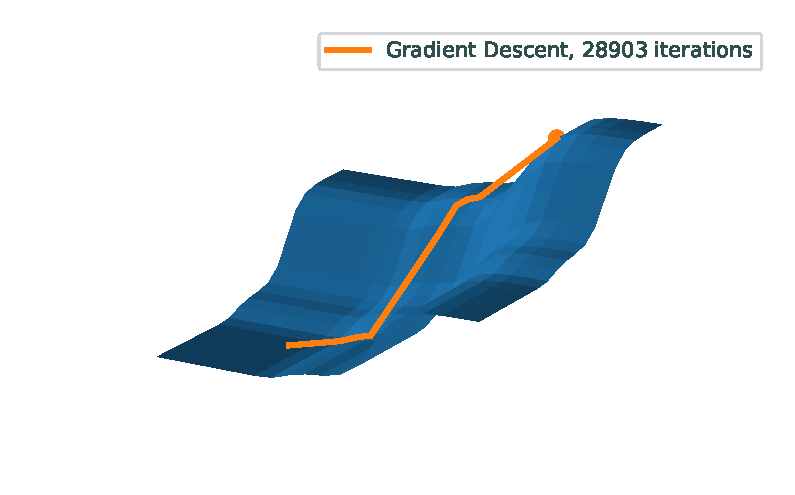
\includegraphics[width=.7\textwidth]{figures/steepest.pdf}
\caption{On this surface, gradient descent takes an extreme number of iterations to converge to the minimum because it gets stuck in the flat basins of the surface.}
\label{basis:steepest}
\end{figure}

Unlike the method of steepest descent, the \emph{conjugate gradient algorithm} chooses a search direction that is guaranteed to be a descent direction, though not the direction of greatest descent.
These directions are using a generalized form of orthogonality called \emph{conjugacy}.

Let $Q$ be a square, positive definite matrix.
A set of vectors $\{\x_0, \x_1, \ldots, \x_m\}$ is called \emph{Q-conjugate} if each distinct pair of vectors $\x_i,\x_j$ satisfy $\x_i\trp Q\x_j = 0$.
A $Q$-conjugate set of vectors is linearly independent and can form a basis that diagonalizes the matrix $Q$.
This guarantees that an iterative method to solve $Q\x = \b$ only require as many steps as there are basis vectors.

Solve a positive definite system $Q\x = \b$ is valuable in and of itself for certain problems, but it is also equivalent to minimizing certain functions.
Specifically, consider the quadratic function
\[
f(\x) = \frac{1}{2}\x\trp Q\x - \b\trp\x + c.
\]
Because $Df(\x)\trp = Q\x - \b$, minimizing $f$ is the same as solving the equation
\[
\0 = Df(\x)\trp = Q\x - \b\quad\Rightarrow\quad Q\x = \b,
\]
which is the original linear system.
Note that the constant $c$ does not affect the minimizer, since if $\x^*$ minimizes $f(\x)$ it also minimizes $f(\x)+c$.

% This technique is very useful for solving large systems of equations in situations where other methods are unsuitable and where the matrix $Q$ is positive definite, which implies invertibility.
% It works equally well for optimizing convex quadratic functions and can be extended to more general non-linear classes of optimization.

% \subsection*{The Algorithm} % -----------------------------------------------

Using the conjugate directions guarantees an iterative method to converge on the minimizer because each iteration minimizes the objective function over a subspace of dimension equal to the iteration number.
Thus, after $n$ steps, where $n$ is the number of conjugate basis vectors, the algorithm has found a minimizer over the entire space.
In certain situations, this has a great advantage over gradient descent, which can bounce back and forth.
This comparison is illustrated in Figure \ref{basis:steepVsConj}.
Additionally, because the method utilizes a basis of conjugate vectors, the previous search direction can be used to find a conjugate projection onto the next subspace, saving computational time.

\begin{figure}[H]
\centering
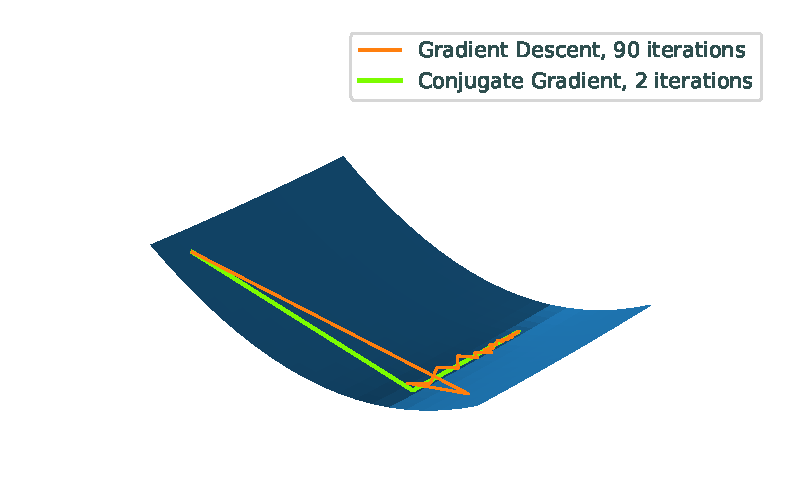
\includegraphics[width=.7\textwidth]{figures/steepVsConj.pdf}
\caption{Paths traced by Gradient Descent (orange) and Conjugate Gradient (red) on a quadratic surface.
Notice the zig-zagging nature of the Gradient Descent path, as opposed to the Conjugate Gradient path, which finds the minimizer in 2 steps.}
\label{basis:steepVsConj}
\end{figure}

% Algorithm \ref{Alg:linear-conjugate-gradient} contains these techniques and outlines an iterative process2 for solving the linear system $Q\x = \b$.

\begin{algorithm}[H]
\begin{algorithmic}[1]
\Procedure{Conjugate Gradient}{$\x_0$, $Q$, $\mathbf{b}$, \li{tol}}
    % \State \textrm{Choose initial point } $\x_0$.
    \State $\mathbf{r}_0 \gets Q\x_0 - \b$
    \State $\mathbf{d}_0 \gets -\mathbf{r}_0$
    \State $k \gets 0$
    \While{$\|\mathbf{r}_k\| \geq $ \li{tol},\ $k < n$}
        \State $\alpha_k \gets \mathbf{r}_k\trp \mathbf{r}_k / \mathbf{d}_k\trp Q\mathbf{d}_k$
        \State $\x_{k+1} \gets \x_k + \alpha_k \mathbf{d}_k$
        \State $\mathbf{r}_{k+1} \gets \mathbf{r}_k + \alpha_k Q\mathbf{d}_k$
        \State $\beta_{k+1} \gets \mathbf{r}_{k+1}\trp \mathbf{r}_{k+1} / \mathbf{r}_k\trp \mathbf{r}_k$
        \State $\mathbf{d}_{k+1} \gets -\mathbf{r}_{k+1} + \beta_{k+1}\mathbf{d}_k$
        \State $k \gets k+1$.
    \EndWhile
    \pseudoli{return} $\x_{k+1}$
\EndProcedure
\end{algorithmic}
\caption{}
\label{Alg:linear-conjugate-gradient}
\end{algorithm}

The points $\x_k$ are the successive approximations to the minimizer, the vectors $\mathbf{d}_k$ are the conjugate descent directions, and the vectors $\mathbf{r}_k$ (which actually correspond to the steepest descent directions) are used in determining the conjugate directions.
The constants $\alpha_k$ and $\beta_k$ are used, respectively, in the line search, and in ensuring the $Q$-conjugacy of the descent directions.

\begin{problem}{Conjugate gradient for linear systems}{}
Write a function that accepts an $n \times n$ positive definite matrix $Q$, a vector $\b\in\mathbb{R}^n$, an initial guess $\x_0\in\mathbb{R}^n$, and a stopping tolerance.
Use Algorithm \ref{Alg:linear-conjugate-gradient} to solve the system $Q\x = \b$.
Continue the algorithm until $\|\mathbf{r}_k\|$ is less than the tolerance, iterating no more than $n$ times.
Return the solution $\x$, whether or not the algorithm converged in $n$ iterations or less, and the number of iterations computed.

Test your function on the simple system
\[
Q = \left[\begin{array}{cc}2 & 0 \\ 0 & 4\end{array}\right],
\qquad
\b = \left[\begin{array}{c}1 \\ 8\end{array}\right],
\]
which has solution $\x^* = \left[\frac{1}{2}, 2\right]\trp$.
This is equivalent to minimizing the quadratic function $f(x,y) = x^2 + 2y^2 - x - 8y$; check that your function from Problem \ref{prob:gradientmethods-steepest-descent} gets the same solution.

More generally, you can generate a random positive definite matrix $Q$ for testing by setting setting $Q = A\trp A$ for any $A$ of full rank.
\begin{lstlisting}
>>> import numpy as np
>>> from scipy import linalg as la

# Generate Q, b, and the initial guess x0.
>>> n = 10
>>> A = np.random.random((n,n))
>>> Q = A.T @ A
>>> b, x0 = np.random.random((2,n))

>>> x = la.solve(Q, b)      # Use your function here.
>>> np.allclose(Q @ x, b)
<<True>>
\end{lstlisting}
\label{prob:gradientmethods-linear-cg}
\end{problem}

\subsection*{Non-linear Conjugate Gradient}
The algorithm presented above is only valid for certain linear systems and quadratic functions, but the basic strategy may be adapted to minimize more general convex or non-linear functions.
Though the non-linear version does not have guaranteed convergence as the linear formulation does, it can still converge in less iterations than the method of steepest descent.
Modifying the algorithm for more general functions requires new formulas for $\alpha_k$, $\mathbf{r}_k$, and $\beta_k$.

\begin{itemize}
\item The scalar $\alpha_k$ is simply the result of performing a line-search in the given direction $\mathbf{d}_k$ and is thus defined $\alpha_k = \underset{\alpha}{\text{argmin}}\ f(\x_k + \alpha \mathbf{d}_k)$.
\item The vector $\mathbf{r}_k$ in the original algorithm was really just the gradient of the objective function, so now define $\mathbf{r}_k = Df(\x_k)\trp$.
\item The constants $\beta_k$ can be defined in various ways, and the most correct choice depends on the nature of the objective function.
A well-known formula, attributed to Fletcher and Reeves, is $\beta_{k} = Df(\x_k)Df(\x_{k})\trp / Df(\x_{k-1}) Df(\x_{k-1})\trp$.
\end{itemize}
%
% Inserting these adjustments to Algorithm \ref{Alg:linear-conjugate-gradient} results in the following routine.

\begin{algorithm}[H]
\begin{algorithmic}[1]
\Procedure{Non-Linear Conjugate Gradient}{$f$,\ $Df$,\ $\x_0$,\ \li{tol},\ \li{maxiter}}
    \State $\mathbf{r}_0 \gets -Df(\x_0)\trp$
    \State $\mathbf{d}_0 \gets \mathbf{r}_0$
    \State $\alpha_0 \gets \underset{\alpha}{\text{argmin}} f(\x_0 + \alpha\mathbf{d}_0)$
    \State $\x_{1} \gets \x_0 + \alpha_0 \mathbf{d}_0$
    \State $k \gets 1$
    \While{$\|\mathbf{r}_k\| \geq$ \li{tol},\ $k < $ \li{maxiter}}
        \State $\mathbf{r}_{k} \gets -Df(\x_k)\trp$
        \State $\beta_{k} = \mathbf{r}_{k}\trp \mathbf{r}_k / \mathbf{r}_{k-1}\trp \mathbf{r}_{k-1}$
        \State $\mathbf{d}_{k} \gets \mathbf{r}_{k} + \beta_{k}\mathbf{d}_{k-1}$.
        \State $\alpha_k \gets \underset{\alpha}{\text{argmin}}\ f(\x_k + \alpha\mathbf{d}_k)$.
        \State $\x_{k+1} \gets \x_k + \alpha_k\mathbf{d}_k$.
        \State $k \gets k+1$.
    \EndWhile
\EndProcedure
\end{algorithmic}
\caption{}
\label{Alg:nonlinear-conjugate-gradient}
\end{algorithm}

\begin{problem}{}{}
Write a function that accepts a convex objective function $f$, its derivative $Df$, an initial guess $\x_0$, a convergence tolerance defaultin to $1e^{-5}$, and a maximum number of iterations defaultin to $100$.
Use Algorithm \ref{Alg:nonlinear-conjugate-gradient} to compute the minimizer $\x^*$ of $f$.
Return the approximate minimizer, whether or not the algorithm converged, and the number of iterations computed.

Compare your function to SciPy's \li{opt.fmin_cg()}.
\begin{lstlisting}
>>> opt.fmin_cg(opt.rosen, np.array([10, 10]), fprime=opt.rosen_der)
<<Optimization terminated successfully.
         Current function value: 0.000000
         Iterations: 44
         Function evaluations: 102>>  # Much faster than steepest descent!
         <<Gradient evaluations: 102>>
array([ 1.00000007,  1.00000015])
\end{lstlisting}
\label{prob:gradientdescent-nonlinear-cg}
\end{problem}


